%================================================================
\chapter{Tools for Analysis}\label{chap:TfA}
%================================================================
In this chapter, we introduce the various numerical methods used for investigating the models used in this thesis. 


%================================================================
\section{Trainability}\label{sec:Trainability}
%================================================================
In machine learning, \emph{trainability} refers to how easily a particular model can be trained under different conditions \cite{abbas2020power}. A common way of to asses the trainability is by exploring the geometry of the loss landscape. For example, the loss function of dense neural networks exhibit local flatness for most directions in parameter space, and strong distortion in others \cite{karakida2019universal}. In a loss landscape that is mostly flat, the gradient of the model tends to diminish, known as \emph{vanishing gradient}, making it difficult to train the model using gradient-based methods. This problem is known to worsen with the number of layers, making the training of deep models prohibitive.

To investigate the flatness and distortions of the loss landscape, a common metric to use is the \emph{Hessian} of the loss, which we will introduce in the next subsection. 
%================================================================
\subsection{Hessian Matrix}\label{sec:HessianMatrix}
%================================================================
Let $f(\boldsymbol{x}^{(k)}; \boldsymbol{\theta})$ be a parameterized and differentiable model, where $\boldsymbol{x}^{(k)} \in \mathbb{R}^p$ are $p$ features, and $\boldsymbol{\theta} \in \mathbb{R}^{n_\theta}$ are $n_{\theta}$ model parameters. For a general loss function on the form \autoref{eq:LossFunction}, $L(\boldsymbol{\theta}) = \sum{_{k=1}^{N}L(f(\boldsymbol{x}^{(k)};\boldsymbol{\theta}), y^{(k)}})$, where $N$ is the number of samples in the data set, the Hessian matrix of the loss function is given by

\begin{equation}
\label{eq:Hessian}
    H_{ij} = \frac{\partial^2 L(\boldsymbol{\theta})}{\partial \boldsymbol{\theta}_i\partial \boldsymbol{\theta}_j}.
\end{equation}

The Hessian matrix is an $n_\theta \times n_\theta$ matrix that quantifies the curvature of the loss function locally in the parameter space at the point of $\boldsymbol{\theta}$. This is an extensively studied quantity in the machine learning community, and it has been used to study the loss landscape both for classical and quantum mechanical machine learning models \cite{LeCun2012, Huembeli_2021}. In particular, its eigenvalue spectrum quantifies the amount of curvature in various directions. Typically for classical neural networks, the spectrum is characterized by the presence of many eigenvalues near zero, with the exception of a few large ones(so-called "big killers")\cite{LeCun2012}. This indicate the that loss landscape is mostly flat, with huge distortions in a few directions, which in turn causes slow optimization as discussed earlier. 

%================================================================
\subsection{Empirical Fisher Information Matrix}\label{sec:EFIM}
%================================================================
An apparent shortcoming of the Hessian matrix \autoref{eq:Hessian} is the large computational cost of computing it, requiring the evaluation of $\mathcal{O}(n_\theta^2)$ double derivatives. This is particularly expensive for models of many parameters, which e.g. neural networks tend to be. An alternative and related quantity, called the \emph{Empirical Fisher Information Matrix}(EFIM)\cite{karakida2019universal}, can be calculated using $\mathcal{O}(n_\theta)$ first order derivatives, which is much better suited for big models. We will now derive the EFIM and relate it to the Hessian.

Assume a square loss $\frac{1}{2N}\sum_{k=1}^{N} (f(\boldsymbol{x}^{(k)}; \boldsymbol{\theta}) - y^{(k)})^2$. Computing \autoref{eq:Hessian} with this loss results in 
    
\begin{equation}\label{eq:HessianSquareLoss}
    H_{ij} = F_{ij} -
    \frac{1}{N}\sum_{k=1}^{N} (y^{(k)} - f(\boldsymbol{x}^{(k)};\boldsymbol{\theta}))\frac{\partial^2 f(\boldsymbol{x}^{(k)};\boldsymbol{\theta})}{\partial \boldsymbol{\theta}_i\partial \boldsymbol{\theta}_j}, 
\end{equation}
where F is identified as the EFIM, given by
\begin{equation}
\label{eq:EmpiricalFisher}
    F_{ij} =  \frac{1}{N}\sum_{k=1}^{N}
    \frac{\partial f(\boldsymbol{x}_k;\boldsymbol{\theta})}{\partial \boldsymbol{\theta}_i}
    \frac{\partial f(\boldsymbol{x}_k;\boldsymbol{\theta})}{\partial \boldsymbol{\theta}_j}.
\end{equation}

From \autoref{eq:HessianSquareLoss}, the EFIM can been seen to coincide with the Hessian matrix if $f(\boldsymbol{x}^{(k)};\boldsymbol{\theta}) = y^{(k)}$, since the terms in the last sum vanishes. This is the case if the model manages to perfectly replicate the targets from the inputs, which is approximately true for well-trained models what fit the data sufficiently. However, even for untrained models, the EFIM is sometimes used as a cheaper alternative to the Hessian matrix, particularly for investigating the geometry of the loss landscape via its eigenvalue spectrum. This has been done both for classical and quantum mechanical machine learning models \cite{karakida2019universal} \cite{abbas2020power}. It is worth pointing out that these investigations, as well as this thesis, are mainly concerned with untrained models. Consequently, the EFIM does not coincide with the Hessian matrix and does not give a mathematically accurate description of the curvature of the loss landscape. However, the EFIM still serves as a heuristic for addressing the flatness and distortions of the loss landscape. 

%================================================================
\section{Expressivity}\label{sec:Expressivity}
%================================================================
\emph{Expressivity} in machine learning, especially in the context of neural networks, is a way of characterizing how architectural properties of a model affect the space of functions it can compute. More simply put, expressivity measures how flexible and complex the model is. The first attempts to measure expressivity of neural networks took a highly theoretical approach, such as \citet{Bartlett} calculating of the VC dimension of shallow neural networks. The VC dimension, or \emph{Vapnik–Chervonenkis} dimension\cite{hastie01statisticallearning}, is a well-established measure of complexity. However, it is known to be hard to compute in practice for a variety of models\cite{abbas2020power}.  

%================================================================
\subsection{Trajectory Length}\label{sec:TrajectoryLength}
%================================================================
In order to explore the expressivity of deep neural networks, \citet{raghu2017expressive} introduced a more practical alternative to VC dimension called \emph{trajectory length}. This is an easy-to-compute heuristic that measures how small perturbations in the input of neural networks grows as it is passed through the various layers of the model. 

Given a trajectory $\boldsymbol{x}(t)$ in a $p$-dimensional space, its arc length 
$l(\boldsymbol{x}(t))$ is given by
\begin{equation}
   l(\boldsymbol{x}(t)) = 
   \int_{t} \big\Vert \frac{\boldsymbol{x}(t)}{dt} \big\Vert dt
\end{equation}
where $\Vert \cdot\Vert$ indicates the Euclidean norm. Conceptually, the arc length of the trajectory $\boldsymbol{x}(t)$ is sum of the norm of its infinitesimal segments. By approximating the trajectory with a finite number of points $\boldsymbol{x}(t_i)$, its arc length can be estimated as 

\begin{equation}\label{eq:TrajectoryLengthDiscrete}
   l(\boldsymbol{x}(t)) \approx 
   \sum_{i=1}^{N-1} \Vert\boldsymbol{x}(t_{i+1}) - \boldsymbol{x}(t_{i})\Vert.
\end{equation}

By making an appropriate trajectory $\boldsymbol{x}(t_i)$ in some input space, it is possible to investigate how its length changes as it is passed through each layer of a neural network. To be concrete, the quantity of interest is $l(\boldsymbol{a}^{l}(t_i))$, where $\boldsymbol{a}^{l}(t_i)$ are the outputs of layer $l$ resulting from the input $\boldsymbol{x}(t_i)$ for some neural network. As an example, one can make a trajectory $\boldsymbol{x}(t_i) \in \mathbb{R}^2$ in the shape of a circle. By projecting $\boldsymbol{a}^{l}(t_i)$ down to 2D, it is possible to visualize how each layer of the neural network distorts the trajectory. This has been exemplified in \autoref{fig:trajectoryLengthExample}.

\begin{figure}[H]
    \centering
    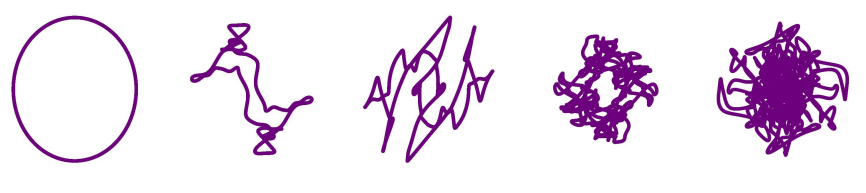
\includegraphics[width=10cm]{latex/figures/trajectoryLengthExample.PNG}
    \caption{Figure showing a trajectory increasing with the depth
of a network. Starting with a circular trajectory (left most
pane), it is fed through a fully connected tanh network with
width 100. Pane second from left shows the image of the circular
trajectory (projected down to two dimensions) after being transformed by the first hidden layer. Subsequent panes show the trajectory after being transformed by multiple layers. This figure is retrieved from \citet{raghu2017expressive}.}
\label{fig:trajectoryLengthExample}
\end{figure}

\autoref{fig:trajectoryLengthExample} shows that the inputs get transformed in a highly non-linear way as it is being transformed by each layer. Especially, neighboring points in the input trajectory gets mapped further and further apart for each transformation, indicating that small perturbations in the input grows for each layer. \citet{raghu2017expressive} showed that the trajectory length of trained neural networks increase exponentially with depth, suggesting a capacity to compute exponentially complex functions as the number of layers increase.

